\documentclass[lettersize,journal]{IEEEtran}

\usepackage{amsmath,amsfonts,amssymb}
\usepackage{array}
\usepackage{stfloats}
\usepackage{url}
\usepackage{graphicx}
\usepackage{cite}
\newtheorem{theorem}{Theorem}
\newtheorem{proposition}{Proposition}
\newtheorem{corollary}{Corollary}
\newtheorem{lemma}{Lemma}
\newtheorem{remark}{Remark}
\hyphenation{op-tical net-works semi-conduc-tor IEEE-Xplore}
\def\BibTeX{{\rm B\kern-.05em{\sc i\kern-.025em b}\kern-.08em
    T\kern-.1667em\lower.7ex\hbox{E}\kern-.125emX}}

\urlstyle{same}
\begin{document}

\title{Multirobot Tracking of Separatrices and
Objective Eulerian Coherent Structures}

\author{Christopher Waight and Christopher A. Kitts,~\IEEEmembership{Senior Member,~IEEE}
\thanks{C. Waight is a PhD Candidate in the Robotic Systems Laboratory, Department of Mechanical Engineering, Santa Clara University, Santa Clara, CA 95053 USA (e-mail: cwaight@scu.edu)}
\thanks{C. A. Kitts is Professor and Director of the Robotic Systems Laboratory, Department of Mechanical Engineering, Santa Clara University, Santa Clara, CA 95053 USA (e-mail: ckitts@scu.edu)}
}
\markboth{IEEE Transactions on Robotics}%
{Waight and Kitts: Multirobot Tracking of Separatrices and Objective Eulerian Coherent Structures}

\maketitle

\begin{abstract}
Short-term transport in a geophysical flow is organized by
instantaneous coherent structures, rotation-dominated cores that
retain material and strain-dominated boundaries across which it
separates. Conventional navigation strategies rely on prescribed
trajectories to survey these domains, while existing robotic trackers
either commit to a presumed structure or pay an integration latency.
This paper instead formulates adaptive navigation as the process of
modifying a multivehicle cluster's motion path based on measurements
taken while moving, using only instantaneous local flow measurements.
To our knowledge, this is the first experimental demonstration of an
objective, model-free coherent structure tracker. A cooperative estimator
recovers the local quadratic field model from one synchronous sample,
with six robots proved minimal. The fit supplies two surrogates: the
Jacobian determinant and the smaller rate-of-strain eigenvalue. We develop
navigation controllers for both and find a tradeoff between objectivity
and noise tolerance. The control primitives are admittedly simple,
reactive, and minimal in size; even in their current form, however, they
are capable of demonstrating a comprehensive suite of critical behaviors.
Deployed on Santa Barbara Channel radar currents, both controllers follow
the same dominant ridge for nearly the full record. Ongoing and future
research activities are targeted to mature these controllers, to verify
and validate them experimentally and in field applications, and to extend
the techniques to three-dimensional fields and vector fields.
\end{abstract}

\begin{IEEEkeywords}
Multirobot Systems, Adaptive Navigation, Coherent Structures,
Okubo-Weiss, Rate of Strain, Objectivity, Cooperative
Estimation, Cluster Space Control
\end{IEEEkeywords}

\section{Introduction}

\IEEEPARstart{S}{hort-term} transport in geophysical flows is organized by instantaneous coherent structures, such as separatrices and objective Eulerian coherent structures. These environmental fronts physically separate distinct fluid regions and govern the transport of material through the domain. Characterization of these dynamic structures is challenging, usually performed manually, limited to localized characterization, and dependent on assumptions about front structure. 

Conventional navigation provides waypoints and a prescribed trajectory to survey a region exhaustively and identify features only afterward. Adaptive navigation is the process of modifying a vehicle's direction or motion path based on measurements taken while moving. Single-vehicle approaches require costly lateral movement to sense local gradients, which causes delays and is detrimental in time-varying fields. Multivehicle approaches share simultaneously collected, spatially distributed measurements, and additionally accommodate vehicle failures and adapt formation size and shape to the spatial frequencies in the field.

These capabilities have widespread application across land, sea, air, and space. In scalar fields, maxima are hot spots and pollutant sources; minima are sinks and marine anoxic zones; contours bound the extent of a field or define a safety perimeter. In vector fields, saddle points are low-energy passages; ridges are resource divides and paths of maximum service availability on departure; trenches are accumulators and paths of minimum exposure on approach. Similarly, eddy centers are mixing cores, convergence zones are debris accumulators, and stagnation points serve as areas of minimal drift for station-keeping operations.

To track these features, our current focus is an adaptive multirobot tracking strategy based on local vector field properties. In \cite{9}, a three-robot cluster estimated the location and type of an isolated critical point from a linear fit of simultaneous local velocity measurements, recovering the feature from instantaneous data alone rather than from an accumulated survey.

Beyond isolated points, there is also utility in tracking extended
features such as fronts, dynamically meaningful lines along which
water masses converge. Coordinated multi-vehicle sampling of such
dynamic ocean features is itself an active area of marine robotics,
spanning drifter-referenced AUV surveys \cite{10}, front-tracking
ASV/AUV teams \cite{11}, and adaptive glider fleets \cite{12}.

Another line of great interest is the separatrix. In steady
two-dimensional flows it is the union of the stable and unstable
manifolds through the saddle points, partitioning the domain into
basins whose trajectories do not mix. Tracking it is relevant to
dispersion modeling, pollutant containment, and coastal sensor
deployment \cite{13,14,15}, and, like the related Okubo-Weiss field used
to classify oceanic mesoscale eddies \cite{16}, it can in principle be
inferred from instantaneous measurements alone.

A line of work on separatrix navigation has equipped robot teams to
track a coherent structure directly in the flow rather than
reconstruct it offline, by straddling a presumed manifold with a small
formation \cite{17,18,19,20} or by accumulating an onboard FTLE
estimate over a finite time horizon \cite{21}. Each approach either
commits to the structure's identity before tracking begins or pays an
integration latency before an estimate exists. The AN approach of this
paper requires neither. Neither prior family is objective under a
rotating observer, and the straddle family reports failure at a saddle
rather than a handling strategy for it; the two trackers developed here
need no integration horizon, commit to no structure in advance, and the
$s_1$ tracker remains objective while traversing and capturing at a
saddle.

This paper makes four contributions. First, a cooperative second-order
estimator that recovers the local quadratic model of a two-component
field from one synchronous sample, with six robots proved minimal for
the unconstrained quadratic model, a conic characterization of the
formations that fail, and exact, heading-isotropic noise gains. Second,
two navigation controllers, the $D$ tracker and the $s_1$ tracker, that
read the two terms of one splitting identity, $D = \omega^2/4 - s_1^2$,
off the same six-robot fit: the $D$ tracker attracts to and traverses
the manifold without committing to an attracting or repelling identity
in advance, while the $s_1$ tracker does the same on the objective
strain eigenvalue, so unlike $D$ it stays valid when a team cannot
certify its own orientation against a trusted external reference
\cite{10,22}. Third, closed-loop
frame equivariance of the $s_1$ tracker, proved and demonstrated in a
rotating-frame experiment, against the $D$ tracker's demonstrated
failure under the same rotation. Fourth, a tradeoff between that
objectivity and noise tolerance, with the mechanism diagnosed down to a
specific estimator channel, and a selection rule for choosing between
the two trackers by field and mission; both trackers are also validated
on real Santa Barbara Channel radar currents.

The remainder of the paper reviews related work, defines system modeling
and estimators (Section~\ref{sec:system_modeling}), and the two controllers
(Section~\ref{sec:controllers}), and reports the deployment results.

\subsection{Related Work}
\label{sec:related_robots}

Haller and Yuan formalized the Lagrangian coherent structure (LCS) as
the generalization of stable and unstable manifolds to flows with
arbitrary time dependence \cite{13}. The standard computable definition,
a ridge of the finite-time Lyapunov exponent (FTLE) field, is given in
\cite{15} on the same double-gyre model used throughout this paper. The
objectivity and Lagrangian/Eulerian tradeoff that bears on any Eulerian
surrogate is developed in \cite{23,24,25}. Velocity-gradient
recovery from sparse trajectories \cite{26} and the strain-spin
decomposition itself \cite{27} remain active adjacent directions. The
instantaneous criteria remain the computable workhorses. Okubo and Weiss
partition a planar flow from the local velocity gradient alone
\cite{28,29}, generalized to three dimensions \cite{30}, refined for
oceanographic use \cite{31}, and used at scale in mesoscale eddy censuses
\cite{16}.

The nearest prior work tracks a coherent structure directly with a
robot formation. Michini et al. bracket a presumed stable or unstable
manifold with three robots using only local velocity measurements
\cite{17}. The strategy extends to $N$ robots \cite{18}, was validated
on micro surface vehicles in a flow tank \cite{19}, and related
flow-based control operates marine robots in gyre-like environments
\cite{20}. Unlike methods that sense only a scalar reduction of the
field \cite{32}, the team here fits the full local quadratic vector
field, so the surrogate's shape, not merely its sign, is available to
the controllers. The straddle family commits to the manifold's identity
before tracking begins, and neither controller nor proof addresses the
saddle point itself, exactly where that identity becomes ambiguous;
\cite{17} itself reports that robots following its strategy tend to
veer away from the tracked LCS as they approach a saddle, since the
flow reverses direction on its far side, in both their flow-tank and
ocean trials. Its robots start on the manifold and are advected.
Kularatne and Hsieh instead compute the local FTLE field on board,
recovering the structure's type at the price of a nonzero integration
horizon \cite{21}. None of these strategies estimates the curvature of
the field itself, which is what fixes not just where a structure lies
but what kind it is and how many branches meet there.

On the estimation side, \"{O}gren, Fiorelli, and Leonard established
cooperative gradient climbing with a formation of mobile sensors
\cite{2}, and Bri\~{n}\'{o}n-Arranz, Renzaglia, and Schenato extended
the idea to the Hessian. Five robots on a ring plus one at the center
recover the gradient and Hessian of a scalar signal in closed form
\cite{6}. McDonald, Kitts, and Neumann developed the complementary
adaptive-navigation primitives that follow scalar-field ridges,
trenches, and saddle points from local differences alone
\cite{3,4,5}. Every one of these formations samples a single signal
channel; a coupled two-component field doubles the estimation problem
to twelve unknowns, which none addresses, and \cite{6}'s fixed
symmetric weights hold only for the ideal ring geometry, where the
estimator here solves at the measured positions and stays exact even
as the formation deforms.

This paper and the critical-point and structure-tracking methods above
\cite{9,17,18,19,20,21} navigate a naturally occurring flow sensed in
situ, unlike the separate literature that builds an artificial vector
field as a synthetic guidance signal for single-robot path following
\cite{33} or obstacle avoidance \cite{34}.

\section{System Modeling and Estimation}
\label{sec:system_modeling}

A planar vector field assigns a velocity vector $\mathbf{v}(\mathbf{p}) = (u(\mathbf{p}), v(\mathbf{p}))$ to each position $\mathbf{p} = (x, y)$. Rather than relying on first-order models that cannot identify curvature, this work estimates the second-order Taylor expansion of the field centered around the cluster centroid $\mathbf{p}_c$. 

The local kinematic properties of the flow are governed by the velocity gradient tensor $\mathbf{J} = \mathbf{S} + \mathbf{W}$, which decomposes into the symmetric rate-of-strain tensor $\mathbf{S}$ and the antisymmetric spin tensor $\mathbf{W}$. The determinant of the Jacobian, $D = \det(\mathbf{J})$, identifies the Okubo-Weiss partition between strain-dominated ($D < 0$) and rotation-dominated ($D > 0$) regions \cite{28,29}. For incompressible planar flows, the exact splitting identity relates the two frames:
\begin{equation}
    D = \frac{\omega^2}{4} - s_1^2,
    \label{eq:splitting}
\end{equation}
where $\omega$ is the vorticity and $s_1$ is the minimum eigenvalue of the strain tensor $\mathbf{S}$. This identity establishes two distinct surrogates for tracking attracting structures: the determinant $D$, which is mathematically simple but frame-dependent, and the strain eigenvalue $s_1$, which isolating the invariant symmetric tensor makes strictly objective across rotating observer frames \cite{24}. The canonical double-gyre flow \cite{15} serves as the primary analytic benchmark throughout this work, providing known bounded regions of $D$ and $s_1$ to validate tracking performance.

To recover the second-order coefficients of the local field, the multirobot cluster synchronously samples the ambient flow. A formation of six robots provides exactly the twelve spatial measurements (two velocity components per robot) required to identify the unconstrained planar quadratic model. The cluster fits the measurements through a single $6 \times 6$ linear inversion. The matrix $\boldsymbol{\Phi}$ is full rank and nonsingular as long as the six sampling points do not lie on a common conic \cite{6}. As established in prior analysis, the closer to singular the matrix is, the worse the estimate becomes. This holds true even if the matrix is square; a circle, for example, has a 0 determinant. The pentagon-plus-center formation used throughout this paper structurally avoids this degeneracy. 

\section{Adaptive Navigation Controllers}
\label{sec:controllers}

Both the $D$ tracker and the $s_1$ tracker operate within a four-layer hierarchical control architecture established in our prior cluster space control studies \cite{3,4,9,36}, shown in Fig.~\ref{fig:control_architecture}. 

\begin{figure}[!t]
    \centering
    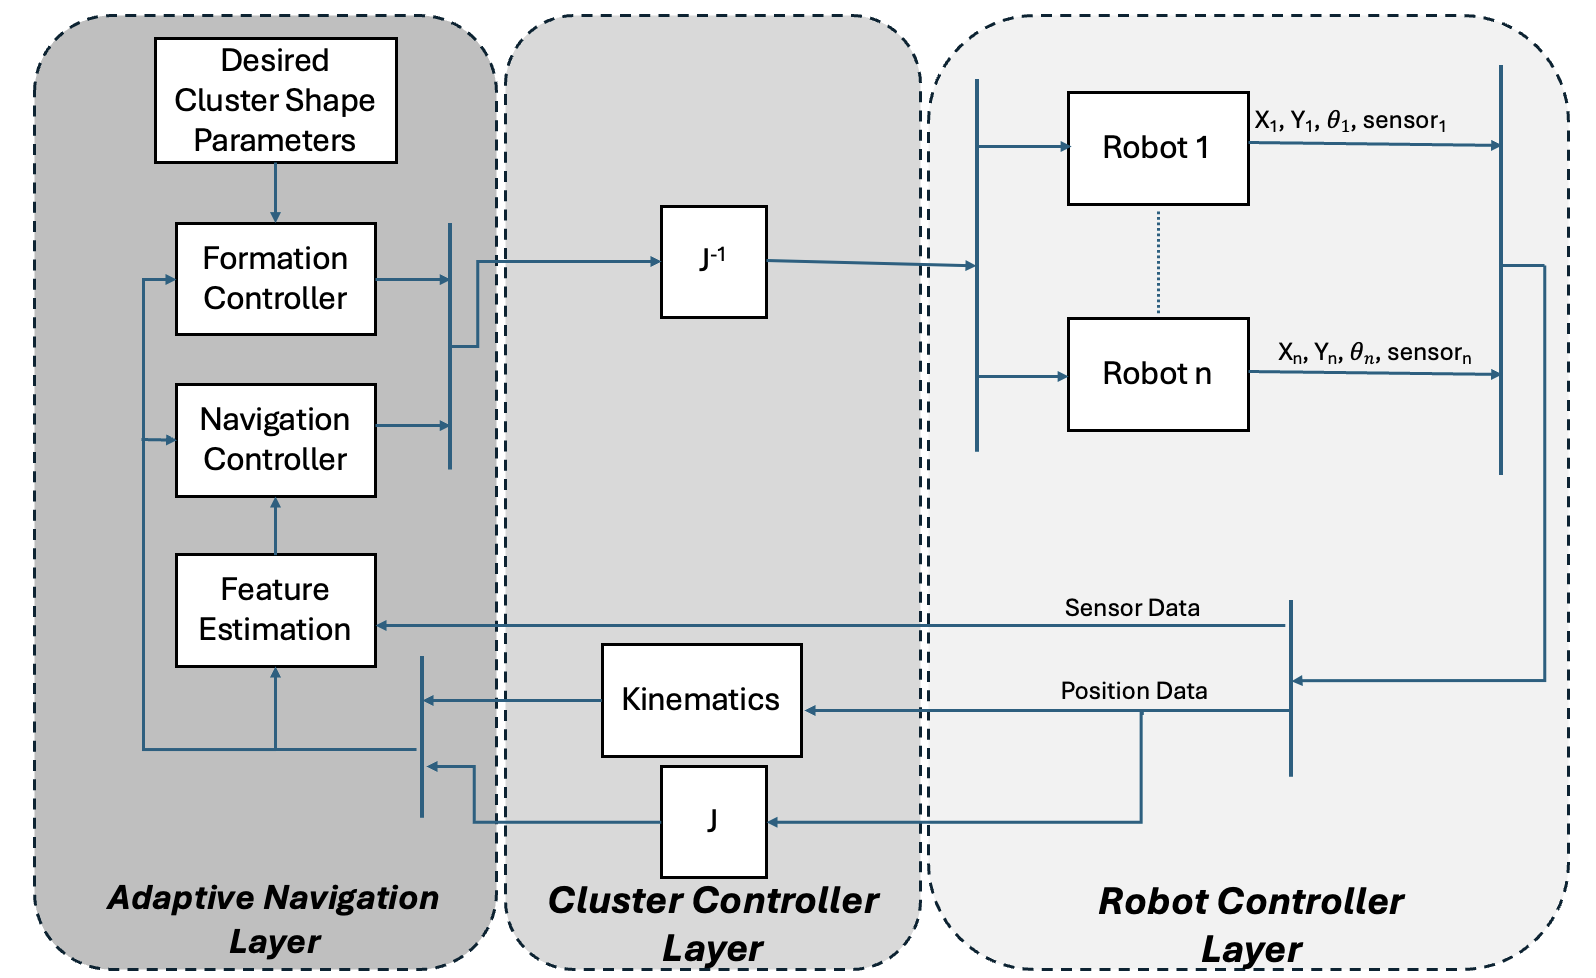
\includegraphics[width=0.40\textwidth]{figures/control_architecture.png}
    \caption{Hierarchical control architecture. Robot controller, cluster controller, and adaptive navigation layers.}
    \label{fig:control_architecture}
\end{figure}

From the bottom up, the robot control layer handles low-level actuation, the cluster space layer maps formation variables through an inverse kinematic Jacobian, the adaptive navigation layer issues the centroid tracking velocity $\dot{\mathbf{p}}_c$, and the state control layer sequences navigation modes and manages hysteresis. This supervisory state machine is the primary mechanism ensuring robust field autonomy.

\subsection{The $D$ Tracker}
The $D$ tracker navigates the separatrix network by driving the cluster centroid onto the trench of the estimated determinant $D$ and then riding the ambient flow along the crest. Utilizing the estimated Hessian $\hat{\mathbf{H}}_D$, the controller executes a saturated Newton step in the transverse direction to seek the trench minimum. Once the cluster is declared on the separatrix—determined by comparing the magnitude of $\hat{D}$ to the local curvature—the along-trench velocity command relies entirely on the measured flow. This combination decoupling ensures rapid convergence across the trench and smooth transport along it, provided the estimated Hessian remains properly conditioned.

\subsection{The $s_1$ Tracker}
The $s_1$ tracker relies entirely on objective quantities, ensuring its command remains invariant under arbitrary rotations of the observer frame. Because the strain tensor does not admit a standard Newton normalization along the trench, both the longitudinal and transverse channels of the $s_1$ tracker are built directly from the estimated gradient $\nabla\hat{s}_1$.

The tangent to the trench is established dynamically by selecting the eigenvector of the strain tensor $\mathbf{S}$ that is least orthogonal to $\nabla\hat{s}_1$. The controller then decouples descent from travel using a projection operator: the transverse channel descends the gradient of $\hat{s}_1$ to lock onto the trench, while the longitudinal channel travels the identified tangent at a bounded cruise speed. This tracking is maintained until the gradient falls below a capture threshold, indicating arrival at a terminal saddle point where the cluster halts.

\section{Simulation Program}
\label{sec:methods}

A Python simulation implementing the 4-layer architecture evaluated both trackers. The double-gyre experiments use the steady field with an explicit Euler integrator at 10~Hz, and robot dynamics following a first-order model. The formation is distributed via the analytic inverse Jacobian. Clean trials and Monte Carlo noise sweeps evaluated the robustness of the trackers across varying field scenarios, tracking start acquisitions, limit cycles, and path adherence against analytic geometry baselines. 

For real-world validation, the simulation processes hourly surface-current frames for the Santa Barbara Channel from the HFRNet U.S.~West~Coast Radial-to-Total Vector product on a $2$~km grid. The setup includes an interpolation block and coordinates mappings to support accurate comparisons with forward-time FTLE fields computed directly from the radar data. Both trackers are tasked with locating and traversing the dominant local ridges.

\section{Results and Discussion}
\label{sec:results}

\subsection{Estimator Accuracy}
\label{sec:results_est}

\begin{figure}[!t]
    \centering
    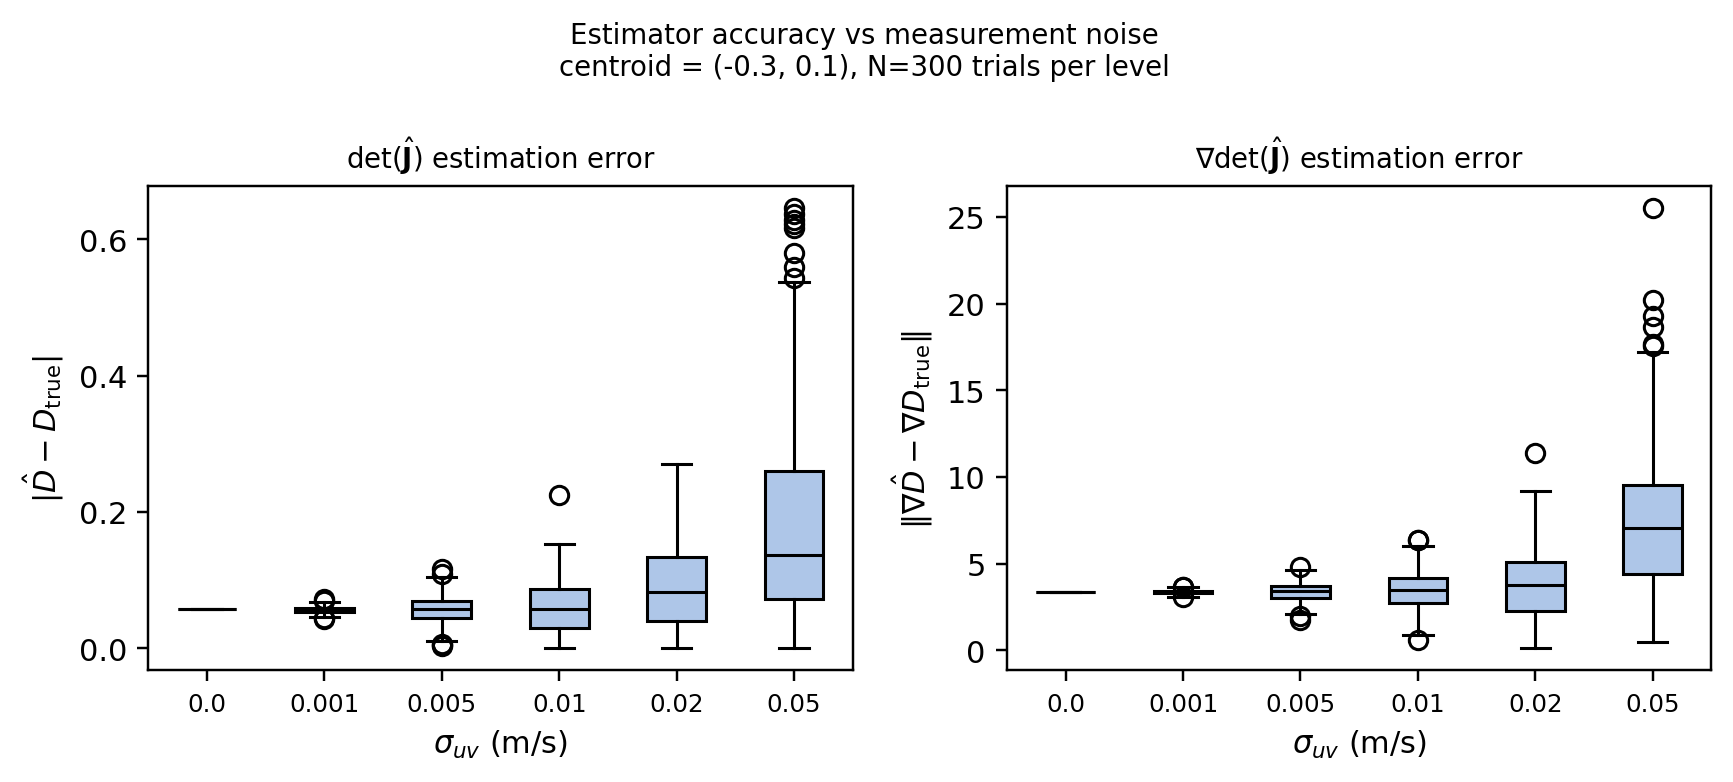
\includegraphics[width=0.9\columnwidth]{figures/estimator_accuracy_vs_noise.png}
    \caption{Estimator accuracy on the steady double gyre at the strain-region
    point $(-0.3, 0.1)$, $10^4$ noise draws per point. (a) Median relative error
    of $\hat{D}$, $\nabla\hat{D}$, and $\hat{\mathbf{H}}_D$ against measurement
    noise at $\rho = 0.075$. The dashed line marks error equal to signal, the
    dash-dotted line the noise at which closed-loop traverse success crosses
    50\%. (b) Mean angle between the fitted and
    the true principal eigenvector of $\hat{\mathbf{H}}_D$, against the
    $45^\circ$ expected of a uniformly random axis. The star is truncation
    acting alone.}
    \label{fig:est_accuracy}
\end{figure}

The estimator was characterized on the steady double gyre before any loop
was closed, over $10^4$ draws per condition at the strain-region point
$(-0.3, 0.1)$. Every theoretical prediction held.
Coefficient standard deviations matched analytical error models within
2.1\%, the reading error induced by position noise matched
kinematic noise bounds within 1.6\%, the downward bias of $\hat{s}_1$ matched
theoretical bias bounds within 5\% in eighteen of twenty-four conditions and
within one standard error of the sample mean in all twenty-four, the six
wider cases being those at $r/\sigma_r \geq 3$ where the predicted bias
is itself below the resolution of $10^4$ draws, and
the signed mean error of $\hat{D}$, $\nabla\hat{D}$, and
$\hat{\mathbf{H}}_D$ was zero to within 2.7\% of one standard deviation
across forty-eight conditions, as unbiasedness requirements dictate.
The correlation between the two component errors at one robot was $0.41$
under position noise against $0.44$ predicted, and zero under measurement
noise, which is the mechanism separating the channels.

In Fig.~\ref{fig:est_accuracy}(a), $\hat{D}$ stays informative to
$\sigma_{uv} \approx 0.07$ and $\nabla\hat{D}$ to $\approx 0.0075$, while
$\hat{\mathbf{H}}_D$ never falls below the error-equals-signal line at any
noise level, held there by $e_H$. In Fig.~\ref{fig:est_accuracy}(b),
truncation acting alone costs the $\hat{\mathbf{H}}_D$ eigendirections
$2.2^\circ$, while noise costs them $24^\circ$ by $\sigma_{uv} = 0.003$ and
$39^\circ$ at the closed-loop failure cliff, against $45^\circ$ for a
uniformly random axis.

The $s_1$ channel was checked at the nominal radius against its analytic
values. The fitted shear strain at three test points is at the $10^{-4}$
level (analytic value zero), and the fitted $\hat{\mathbf{H}}_{s_1}$
eigenvalues are $[-0.011, 0.000]$ and smaller, negative semidefinite as
established limits require. The transverse component of
the estimated gradient at $(0.03, 0.25)$, averaged over ring phase, recovers a
restoring slope of $6.83$ against the analytic transverse curvature
$6.888$, a full-sweep mean of $0.9$\% truncation deficit. The spread
across phases is the expected orientation dependence
rather than scatter. Rotating the ring
through its $72^\circ$ period at the same point moves the recovered slope
between $4.0$ and $9.7$ about that mean of $6.83$, and halving $\rho$ halves
the spread, confirming the linear-in-radius scaling. The mean tracks the
analytic value, so the estimator is not biased in the transverse channel.
An individual formation orientation is. At $\sigma_{uv} = 0.01$ the median
direction error of $\mathbf{e}_2$ is $4.5^\circ$, against $44^\circ$ for
$\nabla\hat{s}_1$ and $41^\circ$ for the $\hat{\mathbf{H}}_D$ eigenvector
($2\times 10^4$ draws per level).

\subsection{Clean Runs}
\label{sec:disc_clean}

\begin{figure}[!t]
    \centering
    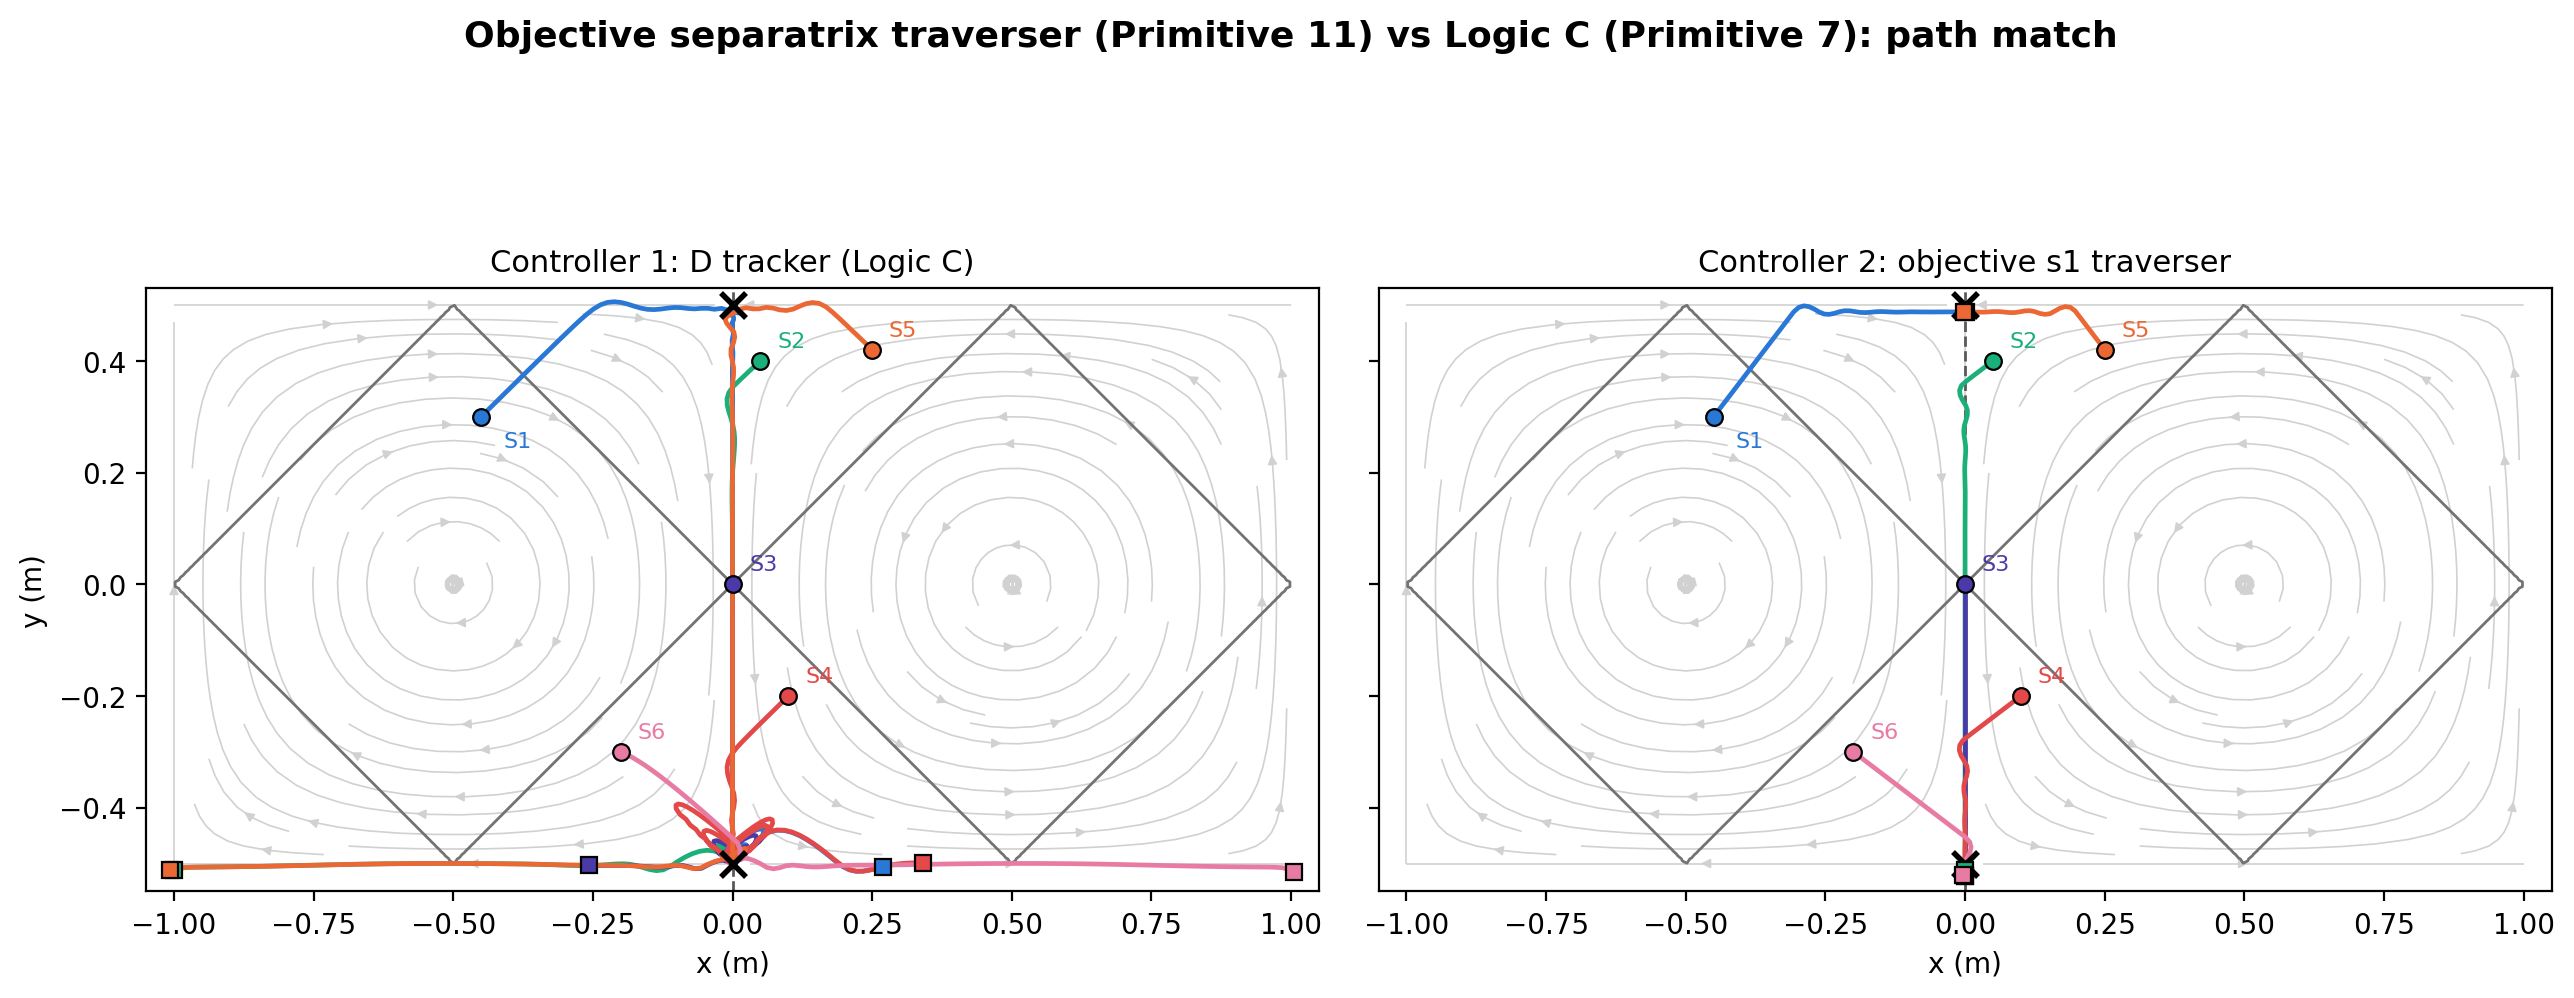
\includegraphics[width=0.44\textwidth]{figures/traverse_vs_logic_c.png}
    \caption{$s_1$ tracker versus $D$ tracker from six matched starts
    ($\bullet$), noise-free, overlaid on the double-gyre streamlines and
    Okubo-Weiss diamonds. Both traverse the same network through the
    isotropic point at the origin. The $s_1$ tracker captures at the
    saddle ($\times$) its tangent orientation resolves toward, while the
    $D$ tracker continues onto the crossing wall trench past every saddle
    it reaches, ending at the square markers.}
    \label{fig:traverse_vs_logic_c}
\end{figure}

Both trackers were run noise-free from the same six starts
(Fig.~\ref{fig:traverse_vs_logic_c}), spanning both gyre halves, the origin,
and points off the structure entirely, between $0$ and $2.7\rho$ from the
nearest trench segment ($\rho = 0.075$, the formation radius). Both acquire
the trench network from every start, in 6 to 35 steps for the $D$ tracker
and 0 to 46 for the $s_1$ tracker, then ride the same segments in the same
direction and cross the isotropic point at the origin. A run acquiring
above the origin therefore rides an attracting OECS to that point and
continues onto a repelling one, on the same law and the same scalar
trench throughout.
The traversal analysis does not distinguish them: the structural normal form
is written for either surrogate and both laws
command the same transverse dynamics. Where the two
commit to the same saddle the paths are visually coincident, and the mean
path gaps of 0.020 to 0.322 over the common on-trench portion
(Fig.~\ref{fig:traverse_vs_logic_c}) open only where they commit to
different ones. Neither needs dedicated machinery at the crossing. The
$s_1$ tracker rides through the origin on the standard tangent selection rule,
and over the sweep of $r_{\text{band}}$ from
0.05 to 0 the degenerate-frame guard never fires once.

By the fourth consequence of the splitting identity, the two trenches
coincide wherever the vorticity vanishes and the flow is
strain-dominated. The double gyre's entire
trench network is such a set, its vorticity
being identically zero on the separatrix
$x_f = 1$ and on all four walls. The lone exception is the isotropic point
at the origin, where $\mathbf{J}$ vanishes entirely and the derivative condition
is unavailable. The six clean runs therefore
agree pointwise for a reason specific to this field, not because the two
surrogates are interchangeable in general.

The trackers part only at the terminal step, and the split is a fact about
the model class rather than about tuning. The $s_1$ tracker settles within
0.011 to 0.022 of a saddle in every run, at whichever one its initial
tangent orientation resolves toward, four at $\mathbf{p}^*_1 = (0, -0.5)$
and two at $\mathbf{p}^*_2 = (0, 0.5)$. The $D$ tracker passes within 0.02
of $\mathbf{p}^*_1$ (closest approach 0.0003--0.0194), then rides onto the
crossing wall trench and continues, because the capture test
$\lambda_1\lambda_2 \geq 0$ cannot fire. This is not a noise floor and not
a tuning margin. By prior derivations, the
fitted $\hat{\mathbf{H}}_D$ is traceless on this field, so its
eigenvalues approximate $\pm|\hat{H}_{xx}|$ on the network, though the
induced trace itself varies with ring phase, from $-0.057$ at the
mirror-antisymmetric phase to $-0.287$ at the worst phase $18^\circ$ away,
a finite-radius truncation artifact. At
the well, at the mirror-antisymmetric ring phase, the estimated pair is
$[-0.51, 0.45]$ against a true $[18.3, 19.2]$; at the worst phase it is
$[-0.72, 0.43]$, which is the floor $e_H$ at $|y| = 0.45$. The same limit binds in
both directions, since $\hat{\mathbf{H}}_{s_1}$ is negative semidefinite
for every field and formation, so neither
surrogate admits a definiteness certificate. The one terminal test a
quadratic fit supports is a vanishing gradient, and a flow saddle is a
genuine two-dimensional minimum of $s_1$, so that test is sufficient
exactly where the $s_1$ tracker needs one and unavailable where the $D$
tracker would need one. Traversal and capture are the same
representability limit read twice.

The clean-field descent also fixes the reachable set, and it is not the
Okubo-Weiss partition. Over a 20\,000-cell start-position grid (distinct
from a separate 20\,000-trial acquisition sweep) no
run settles at a
gyre core, so descent of $\hat{D}$ leaves the rotation-dominated
interiors rather than stalling in them. The reachable set is the
watershed of that descent composited with the flow direction on the
acquired branch, whose arrival rate at $\mathbf{p}^*_1$ is 47.4\% over
that grid and 47.1\% over $n = 10{,}000$ uniformly random starts and
headings. Prior adaptive-navigation primitives \cite{3}, \cite{4} report
local convergence without such an estimate.

\subsection{Controller Robustness and Field Deployments}

On the standard time-varying double gyre \cite{17}, the $D$ tracker reliably acquires and holds the oscillating trench without a feedforward time-derivative term, yielding a maximum transverse offset under $0.015$. However, experiments on a rotating observer frame highlight a key structural divergence: while the $s_1$ tracker maintains perfect objectivity—riding identical material curves across both frames—the $D$ tracker degrades and exits the separatrix entirely due to the artificial additive vorticity of the moving frame.

This trade-off governs deployment. The choice between the trackers depends fundamentally on the sensing capabilities of the robot cluster. The $D$ tracker requires fewer estimation terms and demonstrates an order of magnitude superior robustness to measurement noise, holding the path consistently in high-variance conditions where the $s_1$ tracker's eigenvector comparison collapses. Conversely, the $s_1$ tracker guarantees frame-invariant path adherence, proving strictly necessary if the multirobot team lacks a trusted external reference frame.

Despite these differences, both trackers successfully adapt and respond to real-world data. Driven over measured ocean surface currents spanning a 28-hour HFRNet record in the Santa Barbara Channel, both primitive designs successfully isolate and navigate the single dominant time-invariant ridge structure. Without modification or global knowledge, the team correctly traverses the channel entrance and tracks the structure continuously, establishing a baseline capability for field-ready coherent structure navigation.



\section{Conclusion}
\label{sec:conclusion}

This work presents results of a continuing program to develop multirobot adaptive navigation strategies for environmental feature tracking. We have demonstrated that a six-robot cluster can recover the local quadratic model of a planar flow from a single synchronous sample, supplying both terms of the splitting identity $D = \omega^2/4 - s_1^2$.

Two controllers successfully ride the same trench network from that fit. The $D$ tracker uses a modified Newton step, while the $s_1$ tracker uses the strain term alone. In a rotating-frame experiment, the $s_1$ tracker followed the same material curve in both observer frames, while the $D$ tracker followed a frame artifact. When deployed on real Santa Barbara Channel currents, both trackers successfully followed the same dominant ridge for 28 hours. 

The controllers are admittedly simple, reactive, and minimal in size; even in their current form, however, they are capable of demonstrating a comprehensive suite of critical behaviors for objective, model-free coherent structure tracking. The choice between the two trackers depends on the observing platform: a team that can certify its orientation against a trusted reference should use the $D$ tracker, which tolerates a noisier sensor; a team that cannot should use the $s_1$ tracker, which alone returns the same material curve regardless of frame. 

Ongoing and future work activities are targeted to: a) mature these controllers, b) verify and validate them experimentally and in field applications, and c) extend the techniques to three-dimensional fields and vector fields, and so on.

\begin{thebibliography}{99}
\bibitem{1} J. Cortés and M. Egerstedt, ``Coordinated control of multi-robot
systems: A survey,'' \textit{SICE Journal of Control, Measurement, and
System Integration}, vol. 10, no. 6, pp. 495--503, 2017.

\bibitem{2} P. Ögren, E. Fiorelli, and N. E. Leonard, ``Cooperative control
of mobile sensor networks: Adaptive gradient climbing in a distributed
environment,'' \textit{IEEE Transactions on Automatic Control}, vol. 49, no. 8,
pp. 1292--1302, 2004.

\bibitem{3} R. T. McDonald, C. A. Kitts, and M. A. Neumann, ``Navigation of
scalar fronts with multirobot clusters in simulation and experiment,''
\textit{IEEE Systems Journal}, vol. 14, no. 3, pp. 3755--3766, 2020.

\bibitem{4} C. A. Kitts, R. T. McDonald, and M. A. Neumann, ``Adaptive
navigation control primitives for multirobot clusters: Extrema finding,
contour following, ridge/trench following, and saddle point station keeping,''
\textit{IEEE Access}, vol. 6, pp. 17625--17642, 2018.

\bibitem{5} R. T. McDonald, C. A. Kitts, and M. A. Neumann, ``Experimental
implementation and verification of scalar field ridge, trench, and saddle
point maneuvers using multirobot adaptive navigation,'' \textit{IEEE Access},
vol. 7, pp. 62950--62961, 2019.

\bibitem{6} L. Briñón-Arranz, A. Renzaglia, and L. Schenato, ``Multirobot
symmetric formations for gradient and Hessian estimation with application to
source seeking,'' \textit{IEEE Transactions on Robotics}, vol. 35, no. 3,
pp. 782--789, 2019.

\bibitem{7} M. Mateus, R. Canelas, L. Pinto, and N. Vaz, ``When
tragedy strikes: Potential contributions from ocean observation to
search and rescue operations after drowning accidents,'' \textit{Front.
Mar. Sci.}, vol. 7, art. 55, 2020.

\bibitem{8} P. Keramea, K. Spanoudaki, G. Zodiatis, G. Gikas, and
G. Sylaios, ``Oil spill modeling: A critical review on current trends,
downscaling, and applications,'' \textit{J. Mar. Sci. Eng.}, vol. 9,
no. 2, art. 181, 2021.

\bibitem{9} C. Waight and C. A. Kitts, ``Adaptive navigation of multirobot
systems to critical points in 2D vector fields,'' submitted for publication.

\bibitem{10} J. Das, F. Py, T. Maughan, T. O'Reilly, M. Messié, J. Ryan,
G. S. Sukhatme, and K. Rajan, ``Coordinated sampling of dynamic oceanographic
features with underwater vehicles and drifters,'' \textit{The International
Journal of Robotics Research}, vol. 31, no. 5, pp. 626--646, 2012.

\bibitem{11} S. McCammon, G. Marcon dos Santos, M. Frantz, T. P. Welch,
G. Best, R. K. Shearman, J. D. Nash, J. A. Barth, J. A. Adams, and
G. A. Hollinger, ``Ocean front detection and tracking using a
team of heterogeneous marine vehicles,'' \textit{Journal of Field Robotics},
vol. 38, no. 6, pp. 854--881, 2021.

\bibitem{12} S. R. Ramp et al., ``Preparing to predict: the second autonomous
ocean sampling network (AOSN-II) experiment in the Monterey Bay,''
\textit{Deep Sea Research Part II: Topical Studies in Oceanography}, vol. 56,
no. 3-5, pp. 68--86, 2009.

\bibitem{13} G. Haller and G. Yuan, ``Lagrangian coherent structures and mixing
in two-dimensional turbulence,'' \textit{Physica D: Nonlinear Phenomena},
vol. 147, no. 3-4, pp. 352--370, 2000.

\bibitem{14} T. Peacock and G. Haller, ``Lagrangian coherent structures: The
hidden skeleton of fluid flows,'' \textit{Physics Today}, vol. 66, no. 2,
pp. 41--47, 2013.

\bibitem{15} S. C. Shadden, F. Lekien, and J. E. Marsden, ``Definition and
properties of Lagrangian coherent structures from finite-time Lyapunov
exponents in two-dimensional aperiodic flows,'' \textit{Physica D}, vol. 212,
no. 3-4, pp. 271--304, 2005.

\bibitem{16} C. Dong et al., ``Oceanic mesoscale eddies,'' \textit{Ocean-Land-
Atmosphere Research}, vol. 4, p. 0081, 2025.

\bibitem{17} M. Michini, M. A. Hsieh, E. Forgoston, and I. B. Schwartz,
``Robotic tracking of coherent structures in flows,'' \textit{IEEE Transactions
on Robotics}, vol. 30, no. 3, pp. 593--603, 2014.

\bibitem{18} M. Michini, H. Rastgoftar, M. A. Hsieh, and S. Jayasuriya,
``Distributed formation control for collaborative tracking of manifolds in
flows,'' in \textit{Proc. American Control Conference}, pp. 3874--3880, 2014.

\bibitem{19} M. Michini, M. A. Hsieh, E. Forgoston, and I. B. Schwartz,
``Experimental validation of robotic manifold tracking in gyre-like flows,''
in \textit{Proc. IEEE/RSJ International Conference on Intelligent Robots
and Systems (IROS)}, pp. 2306--2311, 2014.

\bibitem{20} G. Knizhnik, P. Li, X. Yu, and M. A. Hsieh, ``Flow-based control
of marine robots in gyre-like environments,'' in \textit{Proc. 2022 Int. Conf.
on Robotics and Automation (ICRA)}, pp. 3047--3053, 2022.

\bibitem{21} D. Kularatne and M. A. Hsieh, ``Tracking attracting manifolds in
flows,'' \textit{Autonomous Robots}, vol. 41, no. 8, pp. 1575--1588, 2017.

\bibitem{22} R. N. Smith, M. Schwager, S. L. Smith, B. H. Jones, D. Rus,
and G. S. Sukhatme, ``Persistent ocean monitoring with underwater gliders:
Adapting sampling resolution,'' \textit{J. Field Robotics}, vol. 28, no. 5,
pp. 714--741, 2011.

\bibitem{23} G. Haller, ``Lagrangian coherent structures,'' \textit{Annual
Review of Fluid Mechanics}, vol. 47, pp. 137--162, 2015.

\bibitem{24} M. Serra and G. Haller, ``Objective Eulerian coherent
structures,'' \textit{Chaos: An Interdisciplinary Journal of Nonlinear
Science}, vol. 26, no. 5, p. 053110, 2016.

\bibitem{25} P. J. Nolan, M. Serra, and S. D. Ross, ``Finite-time Lyapunov
exponents in the instantaneous limit and material transport,''
\textit{Nonlinear Dynamics}, vol. 100, no. 4, pp. 3825--3852, 2020.

\bibitem{26} T. D. Harms, S. T. M. Dawson, and B. J. McKeon, ``Lagrangian
gradient regression for the detection of coherent structures from sparse
trajectory data,'' \textit{Royal Society Open Science}, vol. 11, no. 9,
p. 240586, 2024.

\bibitem{27} G. Haller, ``Dynamic rotation and stretch tensors from a
dynamic polar decomposition,'' \textit{Journal of the Mechanics and Physics
of Solids}, vol. 86, pp. 70--93, 2016.

\bibitem{28} A. Okubo, ``Horizontal dispersion of floatable particles in the
vicinity of velocity singularities such as convergences,'' \textit{Deep-Sea
Research}, vol. 17, no. 3, pp. 445--454, 1970.

\bibitem{29} J. Weiss, ``The dynamics of enstrophy transfer in two-dimensional
hydrodynamics,'' \textit{Physica D: Nonlinear Phenomena}, vol. 48, no. 2-3,
pp. 273--294, 1991.

\bibitem{30} J. C. R. Hunt, A. A. Wray, and P. Moin, ``Eddies, streams, and
convergence zones in turbulent flows,'' in \textit{Proc. Summer Program,
Center for Turbulence Research}, Rep. CTR-S88, pp. 193--208, 1988.

\bibitem{31} B.-L. Hua and P. Klein, ``An exact criterion for the stirring
properties of nearly two-dimensional turbulence,'' \textit{Physica D}, vol. 113,
no. 1, pp. 98--110, 1998.

\bibitem{32} R. Cooper, D. Rajabhandharaks, R. T. McDonald, M. A. Neumann,
and C. A. Kitts, ``Initial study of multirobot adaptive
navigation for exploring environmental vector fields,'' in \textit{Proc.
IEEE Aerospace Conference}, 2019.

\bibitem{33} W. Yao, H. G. de Marina, B. Lin, and M. Cao,
``Singularity-free guiding vector field for robot navigation,''
\textit{IEEE Trans. Robot.}, vol. 37, no. 4, pp. 1206--1221, 2021.

\bibitem{34} T. Liddy and T.-F. Lu, ``Obstacle avoidance using complex
vector fields,'' in \textit{Proc. Australasian Conf. Robotics and
Automation (ACRA)}, 2008.

\bibitem{35} M. Serra, P. Sathe, I. Rypina, A. Kirincich, S. D. Ross,
P. Lermusiaux, A. Allen, T. Peacock, and G. Haller, ``Search and rescue
at sea aided by hidden flow structures,'' \textit{Nature Communications},
vol. 11, no. 1, p. 2525, 2020.

\bibitem{36} C. A. Kitts and I. Mas, ``Cluster space specification and control
of mobile multirobot systems,'' \textit{IEEE/ASME Transactions on Mechatronics},
vol. 14, no. 2, pp. 207--218, 2009.

\bibitem{37} T. Adamek, C. A. Kitts, and I. Mas, ``Gradient-based cluster space
navigation for autonomous surface vessels,'' \textit{IEEE/ASME Transactions on
Mechatronics}, vol. 20, no. 2, pp. 506--518, 2014.

\bibitem{38} S. Tomer et al., ``A low-cost indoor testbed for multirobot
adaptive navigation research,'' in \textit{Proc. IEEE Aerospace Conference},
pp. 1--12, 2018.

\bibitem{39} C. Waight and C. Kitts, ``A functional indoor testbed for
multirobot adaptive navigation in vector field environments,'' in
\textit{Proc. ASME Int. Design Engineering Technical Conf. and Computers
and Information in Engineering Conf.}, vol. 89251, 2025.

\bibitem{40} NOAA National Centers for Environmental Information,
``Near-real-time surface ocean velocities derived from HF-radar stations
located along coastal waters of North Slope Alaska, Gulf of Alaska,
Puerto Rico/Virgin Islands, eastern U.S./Gulf of America, Hawaii, Great
Lakes, and western U.S.,'' NCEI Accession
gov.noaa.nodc:IOOS-HFRadarRTVector.

\end{thebibliography}

\end{document}
